%%%%%%%%%%%%%%%%%%%%%%%%%%%%%%%%%%%%%%%%%%%%%%%%%%%%%%%%%%%%%%%%%%%%%%%%%%%%%
% Technical report, NeurIPS 2026 formatting.
% Compile:  latexmk -pdf tech_report.tex   (or: pdflatex twice)
%%%%%%%%%%%%%%%%%%%%%%%%%%%%%%%%%%%%%%%%%%%%%%%%%%%%%%%%%%%%%%%%%%%%%%%%%%%%%
\documentclass{article}

% numeric citations, as in the NeurIPS reference style (see the note in the
% conference template); must precede the style file, which loads natbib
\PassOptionsToPackage{numbers, compress}{natbib}
\usepackage[preprint]{neurips_2026}

\usepackage[utf8]{inputenc}
\usepackage[T1]{fontenc}
\usepackage{hyperref}
\usepackage{url}
\usepackage{booktabs}
\usepackage{amsfonts}
\usepackage{amsmath}
\usepackage{amssymb}
\usepackage{nicefrac}
\usepackage{microtype}
\usepackage{xcolor}
\usepackage{graphicx}
\usepackage{listings}

\lstset{
  basicstyle=\ttfamily\footnotesize,
  columns=fullflexible,
  keepspaces=true,
  breaklines=true,
  frame=single,
  framerule=0.4pt,
  rulecolor=\color{gray!60},
  backgroundcolor=\color{gray!8},
  xleftmargin=1.5em,
  xrightmargin=1.5em,
  aboveskip=1.2em,
  belowskip=1.2em,
}

\usepackage{caption}
\captionsetup{font=small}

\title{From Crawl to Corpus: Building, Auditing, and\\
Evaluating a Common Crawl Filtering Pipeline}

\author{%
  Yi Hou \\
  University of Chinese Academy of Sciences\\
  Beijing, China \\
  \texttt{houyi25@mails.ucas.ac.cn}
}

\begin{document}

\maketitle

\begin{abstract}
This report documents a from-scratch pipeline that turns raw Common Crawl WET shards into
language-model pretraining data, and measures what each stage contributes. The pipeline
implements HTML-to-text extraction with encoding detection, fastText language identification,
regular-expression PII masking, Dolma's Jigsaw harmful-content classifiers, the Gopher quality
heuristics, a fastText quality classifier, exact line deduplication, and MinHash+LSH document
deduplication. Applied to 100 WET shards (2.14M documents, 6.2\,GB), it keeps 9.3\% of
documents and yields 340M GPT-2 tokens; line deduplication removes 57.5\% of the lines that
survive language filtering. In a paired 4000-step ablation --- identical initial weights,
identical validation batches --- a model trained on the filtered corpus reaches a 0.27-nat
lower C4-100 validation loss at its best checkpoint (5.64 vs.\ 5.91, perplexity 282 vs.\ 367).
Two caveats bound that number: the quality classifier was selected using positives drawn from
the same benchmark, so part of the gain is agreement with the C4-100 distribution rather than
data quality as such, and the control arm draws from 3$\times$ more tokens, which works
against the filtered arm. Auditing individual samples exposes failure modes that aggregate
statistics hide: the English-trained safety classifiers miss non-English harmful content
entirely, the quality classifier rewards adult pages and pages with residual HTML, and line
deduplication can degrade documents that passed filtering. A scale study closes the loop: at
the 430M-parameter configuration the corpus provides 0.6 tokens per parameter, at
which point both arms memorise the training set (training loss $\approx 0.01$) and validation
loss climbs \emph{above} the uniform-distribution baseline --- so the comparison has to be run
at a smaller model.
\end{abstract}

%=============================================================================
\section{Introduction}

This report implements a pretraining data pipeline from scratch --- HTML-to-text extraction,
language identification, PII masking, harmful-content classifiers, the Gopher quality rules,
a fastText quality classifier, exact line deduplication, and MinHash document deduplication ---
runs it over 100 Common Crawl WET shards, and measures what each stage keeps and what it gets
wrong. The pipeline is evaluated in two ways: by reading individual kept and discarded
documents (§\ref{sec:audit}), and by a paired training ablation that asks whether filtering
improves a language model on the target benchmark (§\ref{sec:ablation}).

Filtering lowers C4-100 validation loss by 0.27 nats at the best checkpoint --- 5.64 against
5.91 for a language-filter-only control, a perplexity of 282 against 367 --- and the gap
widens as training proceeds. Two caveats bound that number, and §\ref{sec:ablation} quantifies
both: the quality classifier was selected using positives drawn from the same benchmark, and
the control arm draws from 3$\times$ more tokens. The first means the gain partly measures
agreement with the C4-100 distribution; the second works against the filtered arm, so the
0.27 nats is a lower bound on the effect of the filtering itself.

%=============================================================================
\section{Experimental setup}
\label{sec:setup}

\paragraph{Data.}
I sample 100 WET shards from the \texttt{CC-MAIN-2026-17} crawl (6.2\,GB compressed,
2{,}135{,}796 documents). I deliberately start from \emph{raw} WET rather than
language-filtered WET, so that language identification is part of the pipeline under study
rather than an assumption. Validation is the C4-100-domains subset of
Paloma~\cite{paloma} (the 100 most common domains in C4, tokenised with GPT-2), which is also
the pipeline's target benchmark.

\paragraph{Benchmark reuse.}
No validation text enters the pretraining corpus, but the benchmark is not held out from the
pipeline either. The quality classifier used for the reported corpus was trained with positives
drawn from the C4-100 validation bin, so the filter was selected to prefer text resembling the
evaluation distribution. The ablation's gain therefore measures agreement with C4-100 as well
as data quality; §\ref{sec:ablation} states that limit next to the result, and
§\ref{sec:quality_clf} describes the stronger design I did not run.

\paragraph{Compute.}
All filtering, deduplication and tokenisation runs on CPU (a 64-core node); training runs on a
single RTX A6000 (48\,GB). The official configuration (batch 128 per device, context 512,
430M parameters) does not fit on a 48\,GB card --- the vocabulary head alone wants
$\approx 0.4$\,MB per token for logits plus softmax, i.e.\ 26\,GB at batch 128 --- so I use
batch 32 with 4 gradient-accumulation steps, which gives the same 65{,}536 tokens per
optimiser step.

\paragraph{Models.}
The ablation compares two data versions under identical training recipes. Because the corpus
is only 340M tokens, the comparison is run with a 30M-parameter model ($d_\text{model}=256$,
4 layers, 4 heads, $d_\text{ff}=1024$); §\ref{sec:ablation} shows why the 430M
configuration is not usable at this data scale.

%=============================================================================
\section{Filtering primitives}
\label{sec:primitives}

Each stage below was implemented from scratch and unit-tested (21 tests across the eight
primitives).

\subsection{HTML to text}
Extraction is \texttt{resiliparse.extract\_plain\_text} over the decoded page, where the
encoding is first guessed with \texttt{detect\_encoding} so that non-UTF-8 pages do not raise.
On the one page I compared against a WET reference, the extracted
text agrees with the reference except for list bullets and breadcrumbs; in general my
extraction keeps slightly more navigation boilerplate than Common Crawl's own extractor, which
the later quality stages are responsible for removing.

\subsection{Language identification}
fastText's \texttt{lid.176.bin} with a 0.7 confidence threshold. On my (unfiltered) shards
only \textbf{30\% of documents are English}, and no other language comes close --- Russian
6.5\%, German 6.0\%, Japanese 5.2\%, Chinese 4.8\%, French 4.6\%, measured on two random samples
of ten shards each --- so language identification is the single largest filter in the pipeline
(§\ref{sec:scale}). Manual inspection of 20 random documents found one clear error (an Italian
page classified \texttt{en} at 0.70, exactly at the threshold); genuinely English pages score
$\geq 0.95$. This is why I keep the threshold at 0.7 but note that short, mixed-language
documents near the boundary are the main source of noise.

\subsection{PII masking}
Three regular expressions replace emails, US phone numbers and IPv4 addresses with
\texttt{|||EMAIL\_ADDRESS|||}-style placeholders. Masking is a transformation, not a filter:
it is applied after the quality decisions so classifiers judge the page as written. Over the
kept corpus it fires 113{,}751 times on phone numbers, 102{,}693 on emails and 7{,}094 on IPs.
The audit (§\ref{sec:audit}) found the main weakness: the phone pattern encodes the US
3-3-4 shape, so international formats (UK \texttt{01923 820644}, Brazilian
\texttt{+55 (11) 98122-2100}, Indian \texttt{+917042230508}) leak through --- 4 of 24 sampled
masked documents. Long digit strings in tables are also false positives.

\subsection{Harmful content}
Dolma's two Jigsaw-trained fastText classifiers~\cite{dolma} (NSFW and hate speech), applied at
a 0.9 confidence threshold. They remove only 0.05\% of documents --- but the audit shows this number
is misleading in two directions. First, both classifiers are trained on English Wikipedia
comments and are \emph{completely blind to non-English harmful content}: a Chinese adult page
scores \texttt{non-nsfw} at 0.974 and \texttt{non-toxic} at 0.991, and is only stopped by
language identification. Second, English adult pages often survive the NSFW threshold with
almost no margin (0.920, 0.915 in two sampled cases; one page scored 0.687 and was stopped only
by the toxicity classifier).

\subsection{Gopher quality heuristics}
Four rules~\cite{gopher} (50--100{,}000 words; mean word length 3--10; at most 30\% of lines
ending in an ellipsis; at least 80\% of words containing a letter) remove 3.5\% of documents,
41.5\% of a raw-CC sample passes. Because the rules assume
whitespace-delimited words, \emph{whole CJK documents fail} the mean-word-length test --- an
artefact of the heuristic, not of the text. And because WET extraction includes sidebar
archive listings, otherwise good blog posts fail the alphabetic-word rule: all four sampled
Gopher rejections failed rule 4 with ratios between 54\% and 72\%, while their prose body was
fine. The rules are useful as a cheap pre-filter, but they are English-specific and they
punish navigation boilerplate rather than content.

\subsection{Quality classifier}
\label{sec:quality_clf}
A fastText classifier trained on positives and negatives (random Common Crawl documents). The
intended positives are external pages cited by Wikipedia; the classifier used for every result
in this report instead uses text drawn from the C4-100 validation bin, because the Wikipedia
link file was never downloaded. The rule followed here is that Paloma may inform filter
construction but may not contribute text to the corpus; even so, it makes the filter and the
benchmark non-independent, and §\ref{sec:ablation} treats that as a caveat on the headline
number. The classifier removes the largest share of \emph{content} filtering: 16.8\% of
documents, second only to language identification. It is also the least reliable component I
built. Because it was trained against a proxy for quality, it has no notion of \emph{harm}:
it assigns \texttt{wiki} at 0.61--0.76 to explicit English adult pages (which only the safety
classifiers then remove), 0.975 to a page whose text still contains raw \texttt{<p>} and
\texttt{<img>} tags, and \texttt{cc} at 0.85--0.93 to clean marketing and conference pages that
it drops --- while a near-identical marketing page survives in the kept set at 0.79. Its
decisions in the 0.5--0.8 band are noisy on this kind of page.

%=============================================================================
\section{Deduplication}
\label{sec:dedup}

\paragraph{Exact line deduplication.}
Two passes over the corpus: count each line's hash, then rewrite every document keeping only
lines whose count is one. Across the 100-shard corpus this removes \textbf{19.0M of 33.0M
lines (57.5\%)} and empties 2{,}550 documents that consisted entirely of template text. This is
the single largest redundancy reduction in the pipeline --- navigation bars, footers and
boilerplate are near-universal --- and it costs one hash-table pass.

\paragraph{MinHash + LSH document deduplication.}
Documents are normalised (NFD, accents stripped, lowercased, punctuation removed, following
the RefinedWeb recipe~\cite{refinedweb}), converted to word 5-gram sets, and summarised as
128-permutation MinHash signatures; locality-sensitive hashing~\cite{mmds} proposes candidate
pairs, whose \emph{true} Jaccard similarity decides the merge (threshold 0.8), and connected
components keep one document each. On my filtered corpus this
removes 52 of 196{,}214 documents (0.03\%): once language, quality and line filtering have run,
almost no near-duplicate documents remain. On this pipeline its contribution is small; it
matters on unfiltered corpora, which is what its fixtures test.

\paragraph{Making MinHash scale.}
The textbook implementation (k independent hash functions per n-gram) was roughly 25$\times$
too slow and 10$\times$ too memory-hungry for a corpus of millions of documents; three changes
fixed it.
First, each n-gram is hashed \emph{once} and the $k$ MinHashes are derived by linear
permutations $(a_j h + b_j) \bmod 2^{31}$ with odd $a_j$ (a bijection, hence as uniform as
independent hash functions) --- this alone took the full corpus from an estimated 8 hours to
20 minutes. Second, signatures are stored as an int32 matrix rather than lists of Python ints
(4 bytes versus $\approx 36$ bytes per value). Third, LSH buckets store a single document id
until a second one collides, and band keys are raw bytes; the number of buckets is
documents\,$\times$\,bands, which makes this the dominant memory term. Measured on a synthetic
100k-document corpus: 89\,s and 0.11\,GB peak RSS, i.e.\ $\approx 89$ minutes and 6.3\,GB
projected for 6M documents.

%=============================================================================
\section{Pipeline output and cost}
\label{sec:scale}

Running the full pipeline over the 100 shards gives the funnel in Table~\ref{tab:funnel}. The
chain runs language identification, then the Gopher rules, the two safety classifiers, the
quality classifier and finally PII masking; each document is attributed to the first stage that
rejected it, so the counts do not double-count. (The table is ordered by how many documents
each stage removes, not in chain order.)

\begin{table}[t]
\caption{Filtering funnel over 100 raw Common Crawl WET shards (2{,}135{,}796 documents).
Language identification dominates because the input is unfiltered; on an
already-English-filtered corpus the quality classifier and the Gopher rules carry most of the
load.}
\label{tab:funnel}
\centering
\begin{tabular}{lrr}
\toprule
Stage & Documents dropped & Share \\
\midrule
Language identification (not English / $<$0.7) & 1{,}501{,}748 & 70.3\% \\
Quality classifier (\texttt{cc} or $<$0.5)      & 359{,}725   & 16.8\% \\
Gopher heuristics                             & 74{,}453    & 3.5\% \\
NSFW classifier                               & 626         & 0.03\% \\
Toxic-speech classifier                       & 480         & 0.02\% \\
\midrule
\textbf{Kept}                                 & 198{,}764   & \textbf{9.3\%} \\
\bottomrule
\end{tabular}
\end{table}

The kept documents then pass line deduplication (57.5\% of lines removed, 2{,}550 documents
emptied) and document deduplication (52 documents removed) before being tokenised with the
GPT-2 tokenizer, one \texttt{<|endoftext|>} per document. (PII masking is applied during
filtering, not here.) The result is \textbf{340{,}133{,}734 tokens} (0.34B) --- 3.1$\times$
fewer bytes than the filtered JSONL it came from.

\paragraph{Cost.}
Filtering 100 shards takes 8 minutes wall-clock with 12 worker processes, each of which loads
$\approx$2.2\,GB of fastText models; deduplication takes 6 minutes; tokenisation takes
57 seconds. Extrapolating linearly, a full 2500-shard corpus (157\,GB) would take roughly 3.5
hours to download, 3.5 hours to filter, 2.5 hours to deduplicate and 25 minutes to tokenise ---
about 10 hours, mostly unattended --- and would yield $\approx$8.5B tokens, against a nominal
8.6B-token budget.

%=============================================================================
\section{Auditing the pipeline output}
\label{sec:audit}

To check individual decisions rather than totals, I drew random samples of kept documents
(from the final corpus) and of discarded and PII-modified documents (by re-running the filter
chain on raw shards) and read them, with the filter scores recomputed for each sample. The
audit is qualitative and the samples are small (8 kept, 20 discarded, 24 masked). Reading 25
raw WET records before any filtering sets the baseline expectation: about half are
machine-generated SEO, adult or gambling pages, and only roughly one in five resembles a
genuine article. Four findings from the filtered samples stood out.

\paragraph{The quality classifier is not a safety filter.}
Sampled English adult pages receive \texttt{wiki} at 0.61--0.76 --- well inside the kept band
--- and are stopped only by the safety classifiers, which in one case held a margin of 0.02.
Non-English adult content is stopped only by language identification.

\paragraph{HTML residue survives extraction.}
A kept page contains raw \texttt{<p>}, \texttt{<span>} and \texttt{<img>} tags plus a
\texttt{[HTML TAGS REMOVED]} placeholder that my own code never emits (it arrives with the WET
text); the same phenomenon is measurable in the provided example WET (94 \texttt{<p>} and 276
\texttt{<br>} tags). The quality classifier scores this page 0.975.

\paragraph{Deduplication can degrade documents after they were filtered.}
Line deduplication rewrites documents \emph{after} the quality decisions, so a page can pass
filtering and then lose the lines that made it substantive. Two sampled documents now have
45 words, or 36.8\% of their lines ending in ``\ldots'' --- both would fail the Gopher rules
they passed earlier.

\paragraph{Phone masking is US-only.}
As noted in §\ref{sec:primitives}: 4 of 24 sampled modified documents retain international
phone numbers, and partial matches can leave fragments such as \texttt{+91-}.

Three cheap fixes follow, and each addresses one of the findings above: a domain blocklist, for
the pages the safety classifiers cleared by 0.02; a residual-HTML check, which no stage performs
today; and a re-run of the length and ellipsis rules after deduplication, which changes the
statistics those rules were applied to.

%=============================================================================
\section{Does filtering pay off?}
\label{sec:ablation}

To test whether the pipeline improves the data rather than merely changing it, I trained two
models on the same 100 shards: one on the full pipeline output (340M tokens) and one on a
control that applies \emph{only} language identification (1.01B tokens) --- the standard
``English Common Crawl'' baseline. The arms share the training recipe, and because both seeds
are fixed they also share the initial weights and the validation batches; at step 0 the two
validation losses agree to every printed digit. The treatment is a bundle --- quality
classifier, Gopher rules, safety classifiers, line deduplication, MinHash deduplication --- so
this experiment measures the bundle rather than any single stage, and the two corpora differ in
size as well as in filtering. Both differences work against the filtered arm, which makes 0.77
passes over its corpus to the control's 0.26; the gap below is a lower bound.

\begin{figure}[t]
\centering
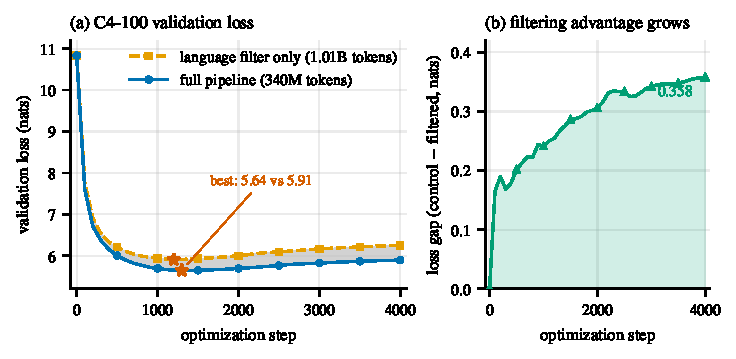
\includegraphics[width=\linewidth]{figures/ablation_30m.pdf}
\caption{\textbf{Filtering the crawl lowers C4-100 validation loss.} Two 30M-parameter models
trained on the same 100 WET shards for 4000 steps (32\,$\times$\,4 gradient accumulation
$=$ 65{,}536 tokens/step): one on the full pipeline (340M tokens), one on a
language-filter-only control (1.01B tokens). (a) Validation loss on the C4-100 domains subset of
Paloma; stars mark each arm's best checkpoint (5.64 vs.\ 5.91 nats). (b) The gap between the
two curves, widening from 0.20 to 0.36 nats. The arms share initial weights and validation
batches, so the two curves are paired; each is nevertheless a single run, with no seed
replicates. Both validation minima fall in the same 1200--1300 step window, after which both
curves rise slowly.}
\label{fig:ablation}
\end{figure}

The filtered corpus reaches a best validation loss of \textbf{5.641} against \textbf{5.906} for
the control: 0.265 nats, a perplexity of 282 against 367. The gap widens steadily with
training, from 0.20 nats at step 500 to 0.358 at step 4000, and it is much larger than the
run's own variability --- the residual scatter of the gap curve is below 0.01 nats, some 30--50 times
smaller than the effect at the best checkpoint. Two secondary observations point the same way
without carrying the argument on their own. The control's \emph{training} loss falls below the
filtered arm's from step 300 onward (3.30 versus 3.72 at the end), consistent with redundant
text being easier to fit. And both validation curves bottom out in the same 1200--1300 window
before rising slowly, which bounds how much of the later gap can be attributed to data quality
rather than to how closely each corpus resembles C4-100.

\begin{figure}[t]
\centering
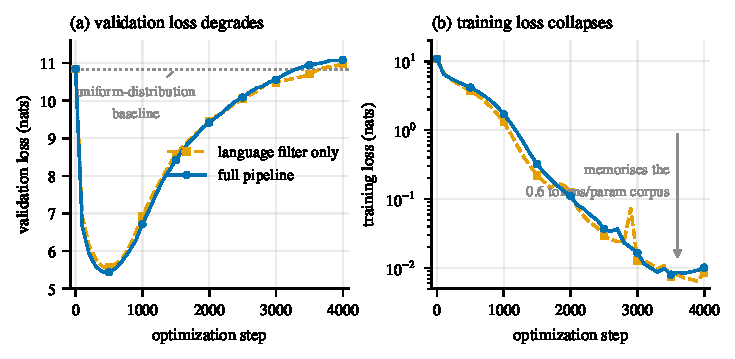
\includegraphics[width=\linewidth]{figures/ablation_430m.pdf}
\caption{\textbf{The same comparison at the 430M-parameter configuration}
(0.6 tokens seen per parameter, against $\approx$20 in the regime it was designed for).
(a) C4-100 validation loss falls until step 500 and then rises, ending above the
uniform-distribution baseline $\ln 50257 = 10.82$. (b) Training loss drops to $\approx 0.01$:
both arms have memorised the tokens they saw. The arms' ordering reverses at step 2200; no
data-quality conclusion can be drawn at this ratio, which is why Figure~\ref{fig:ablation}
uses a 30M-parameter model.}
\label{fig:scale}
\end{figure}

\paragraph{At 430M parameters the ablation measures memorisation, not data quality.}
My first attempt ran a 430M-parameter model on the same data
(Figure~\ref{fig:scale}). Both arms memorised the corpus: training loss fell to 0.01 while
validation loss climbed to 11.0, above the uniform-distribution baseline of 10.82. The model
saw 262M training tokens at 430M parameters --- 0.6 tokens per parameter, against the
$\approx$20 the configuration was designed for (8.6B tokens). The arms do separate early: the
filtered arm leads at every checkpoint up to step 2100, by 0.12 nats at the validation
minimum. But the ordering reverses after step 2200 as each arm memorises its own corpus, so no
data-quality reading is available at this scale and none is claimed here. The 30M-parameter
run above is the primary result, and the lesson is narrow: size a data ablation to the token
budget rather than to the production configuration.

%=============================================================================
\section{Lessons learned}

\begin{itemize}
  \item \textbf{Cheap stages do most of the removal.} Language identification and line
  deduplication account for 70.3\% of the documents and 57.5\% of the lines dropped; the
  classifiers that follow see 26\% of the input. This ablation tested the bundle as a whole, so
  that ordering is an observation about the funnel, not a causal claim.
  \item \textbf{Measure the pipeline at the sample level, not only in aggregate.} Every
  qualitative failure I found (a safety classifier that misses non-English harm, a quality
  classifier that likes adult pages, HTML residue, US-only phone patterns, dedup that
  degrades documents) was invisible in the funnel table.
  \item \textbf{One safety classifier per page is a single point of failure.} Sampled adult
  pages cleared the NSFW threshold by as little as 0.02, while the quality classifier scored
  them \emph{kept}. A domain blocklist costs nothing and would have caught them.
  \item \textbf{Data and model scale are coupled.} The same ablation that separates two corpora
  at 8.7 tokens seen per parameter is uninformative at 0.6, where both arms memorise. Choose
  the ablation model by the token budget, not by the production configuration.
  \item \textbf{Deduplicate before, or re-check after.} Removing shared lines changes document
  statistics; length- and structure-based filters that ran earlier may no longer hold.
\end{itemize}

%=============================================================================
\section{Reproducibility}

The pipeline is a Python package (\texttt{lm\_data}) with 21 unit tests; the corpus build is
four scripts, of which the download stage skips files it already has and the rest can be
re-run per stage:

\begin{lstlisting}[language=bash]
python scripts/download_wet.py --count 100 --output-dir shared-data/raw-wet   # 6.2 GB
python scripts/filter_data.py  --wet-dir shared-data/raw-wet \
        --output-dir shared-data/filtered --workers 12                       # 8 min
python scripts/deduplicate_data.py --input-dir shared-data/filtered \
        --output-dir shared-data/deduped --workers 16                        # 6 min
python scripts/tokenize_data.py --input-dir shared-data/deduped/2_minhash_dedup \
        --output shared-data/train.bin --workers 16                          # 57 s
\end{lstlisting}

The ablation is \texttt{scripts/train\_ablation.py}: the baseline model, optimiser and
schedule, unchanged --- AdamW at lr $6\times10^{-4}$ with 3\% warmup and cosine decay, weight
decay 0.1, gradient clipping at 1.0 --- plus gradient accumulation (32\,$\times$\,4), validation
every 100 steps over 100 batches of 32 sequences drawn from a 9.8M-token Paloma bin under a
fixed seed, and a wall-clock cap. The control corpus is produced by the same filter script with
\texttt{--only-langid}. Figures are regenerated by \texttt{report/make\_figures.py} from the
committed CSVs in \texttt{report/measurements/}. Two environment notes for anyone
re-running this: fastText requires NumPy\,$<$\,2 (its \texttt{predict} path calls
\texttt{np.array(\dots, copy=False)}), and the pipeline's dedup stage drops documents whose
text normalises to nothing --- pure CJK or Cyrillic pages, which \texttt{normalize\_text}
strips to the empty string --- from the similarity computation rather than letting their
identical signatures collide.

\bibliographystyle{plainnat}
\begin{thebibliography}{9}
\bibitem{dolma} L.~Soldaini et al. Dolma: An Open Corpus of Three Trillion Tokens for
Language Model Pretraining Research. \emph{arXiv:2402.00159}, 2024.
\bibitem{gopher} J.~W.~Rae et al. Scaling Language Models: Methods, Analysis \&
Insights from Training Gopher. \emph{arXiv:2112.11446}, 2021.
\bibitem{paloma} I.~Magnusson et al. Paloma: A Benchmark for Evaluating Language Model
Fit. \emph{arXiv:2312.10523}, 2023.
\bibitem{refinedweb} G.~Penedo et al. The RefinedWeb Dataset for Falcon LLM:
Outperforming Curated Corpora with Web Data, and Web Data Only. \emph{arXiv:2306.01116}, 2023.
\bibitem{mmds} J.~Leskovec, A.~Rajaraman, J.~D.~Ullman. \emph{Mining of Massive
Datasets}, 2nd ed. Cambridge University Press, 2014. (Ch.~3: MinHashing and LSH.)
\end{thebibliography}

\end{document}
